%!TEX root = ../thesis.tex
\chapter{Experiments}\label{chap:Experiments}
The amount of experiments, data and visualizations created in this project are more than a dedicated reader is confortable reading in one single pass. For this reason, the experiments and results in this chapter first presented with a simple example, the EmoLex. This example will guide the reader through the methodology to analyze the datasets, and introduce the intuitions presented through simpler visualizations with lesser data. With this intuitions in mind, the results of the other datasets, and language models are presented. In this way, the EmoLex works not only as an introduction to the methodology and results, but also as a lax baseline.

\section{EmoLex}\label{sec:EmoLex}
As an introductory experiment, EmoLex has been embedded into the abstract vector representation of the GloVe language model. This model was selected due to its one-to-one relation between word and embedding, and it's context indepedence. This means that a word will get one single embedding no matter what other words apear next to it. This in comparison to BERT, where the embedding of a single word deppends on the tokens, words, and sentences that come with it. The EmoLex has single words related to emotions, so it must be noted that this experiment and it's results relate to word embedding, and not sentence embedding.

\subsection{Correlational Analysis}

\begin{figure}[H]
  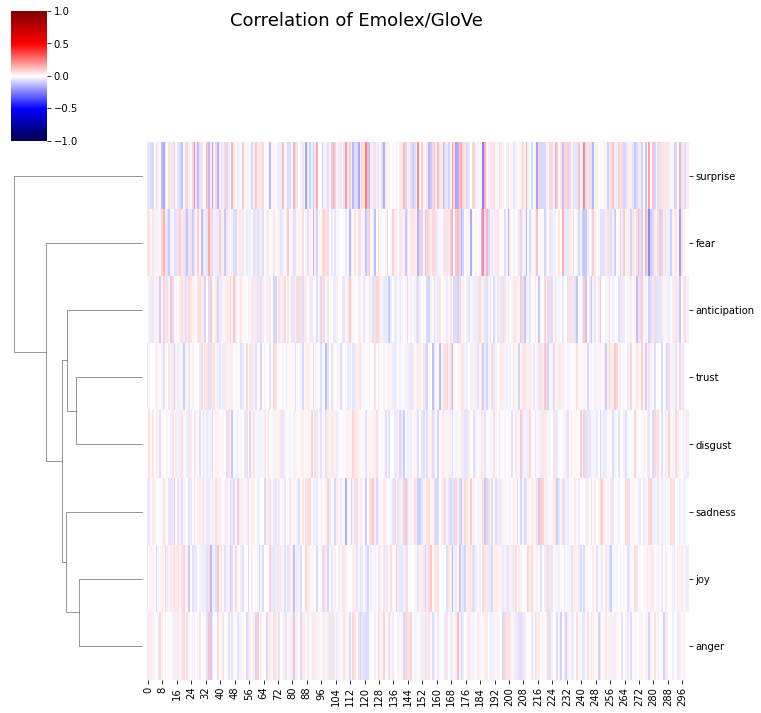
\includegraphics[width=\textwidth]{plots/emolex/cor_emolex_GloVe}
  \centering
  \caption{Emolex Correlation Plot}
\end{figure}\label{fig:cor_emolex_GloVe}

\begin{figure}[H]
  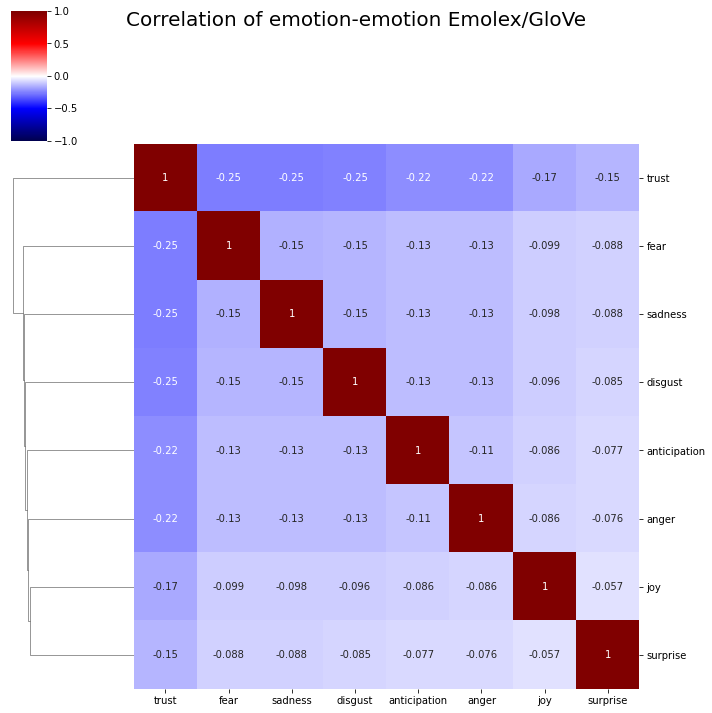
\includegraphics[width=1	extwidth]{plots/emolex/cor_emolex_GloVe_e_e}
  \centering
  \caption{Emolex Correlation Plot}
\end{figure}\label{fig:cor_emolex_GloVe_e_e}

\subsection{PCA}

\begin{figure}[H]
  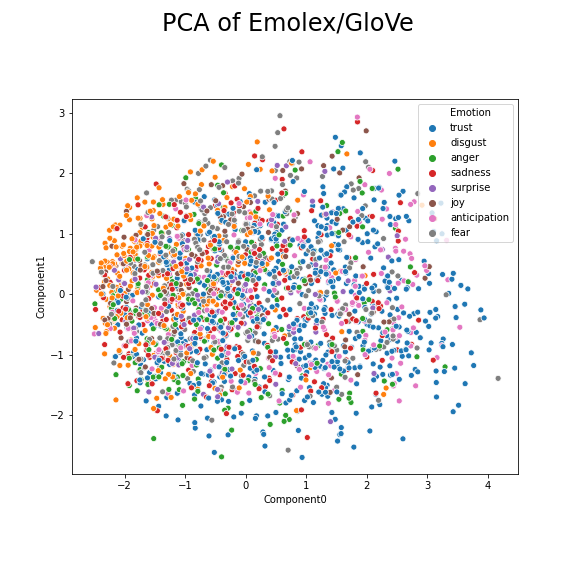
\includegraphics[width=1	extwidth]{plots/emolex/pca_scat_emolex_glove}
  \centering
  \caption{Emolex Scatter plot of PCA}
\end{figure}\label{fig:pca_scat_emolex_glove}

\begin{figure}[H]
  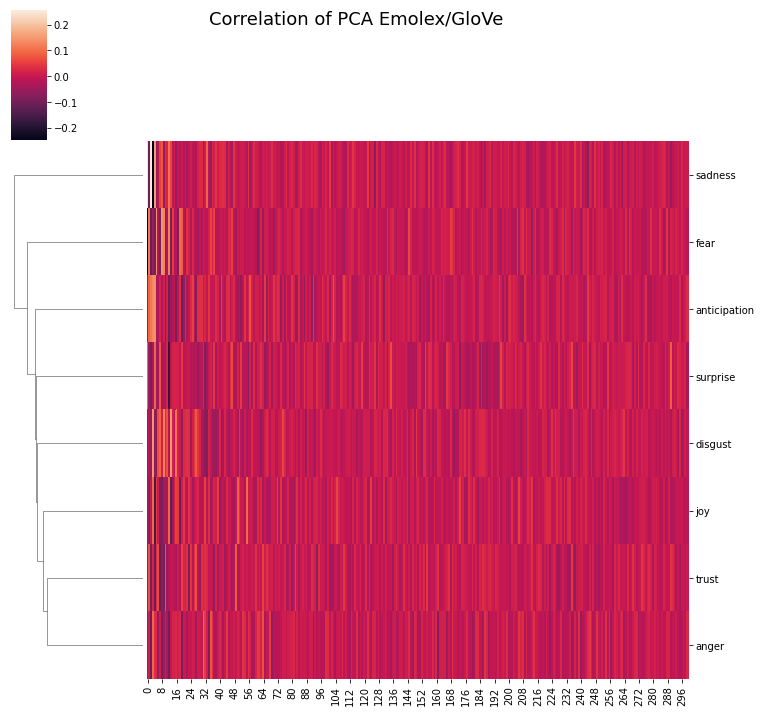
\includegraphics[width=1	extwidth]{plots/emolex/pca_cor_emolex_glove}
  \centering
  \caption{Emolex Correlation of PCA components}
\end{figure}\label{fig:pca_cor_emolex_glove}

\subsection{TSNE}

\begin{figure}[H]
  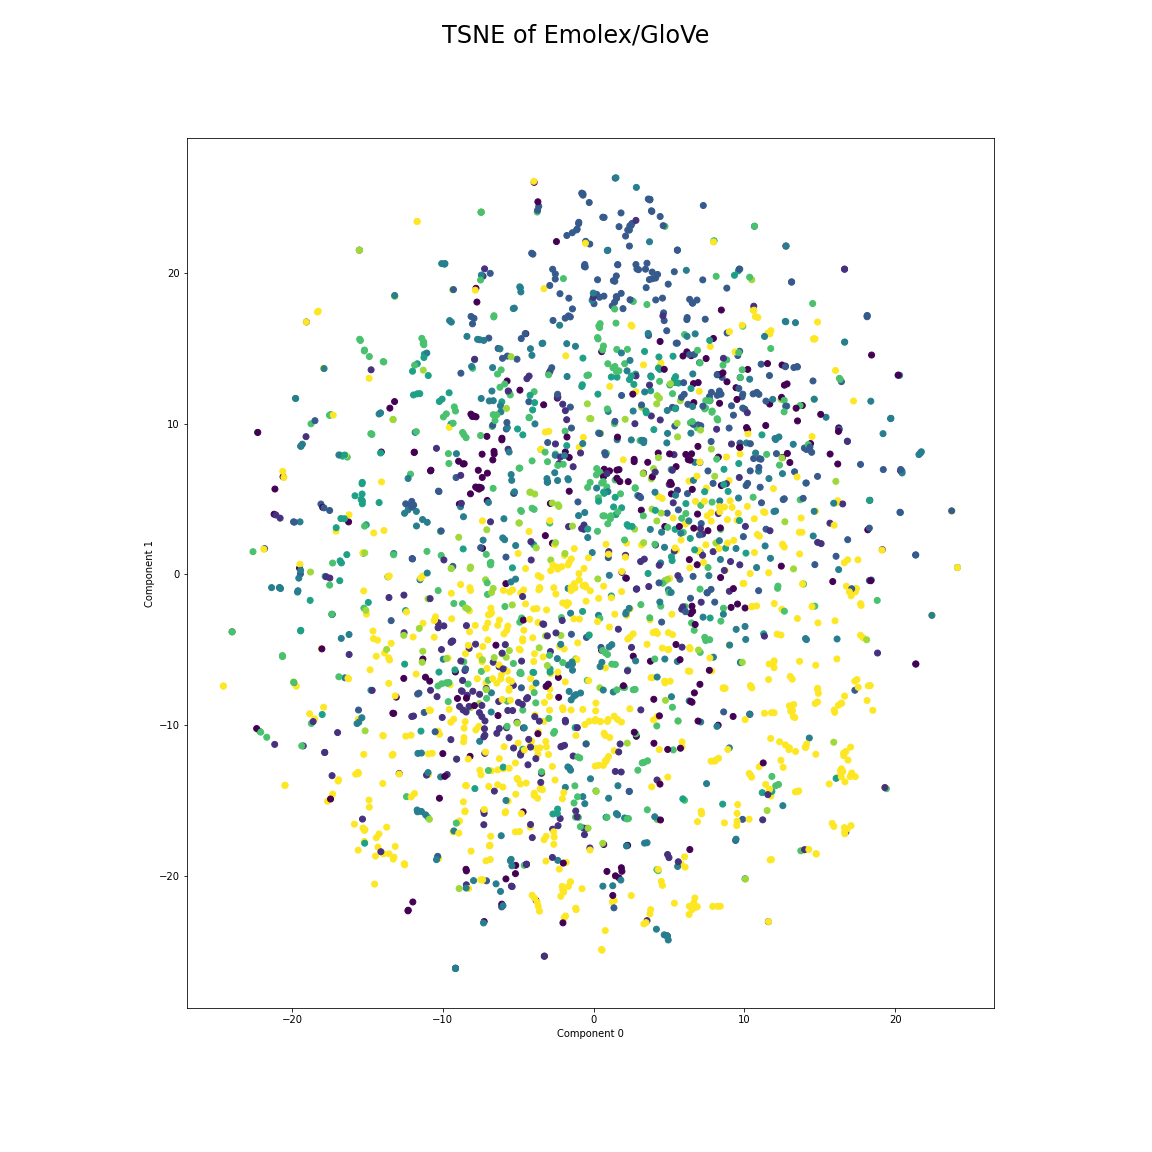
\includegraphics[width=1	extwidth]{plots/emolex/tsne_scat_emolex_glove}
  \centering
  \caption{Emolex Scatter plot of TSNE}
\end{figure}\label{fig:tsne_scat_emolex_glove}

\begin{figure}[H]
  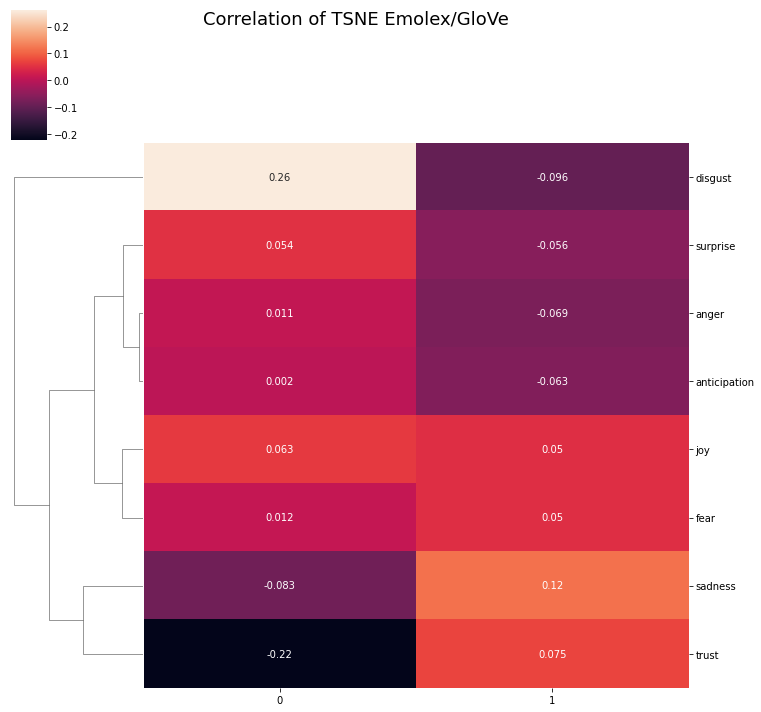
\includegraphics[width=1	extwidth]{plots/emolex/tsne_cor_emolex_glove}
  \centering
  \caption{Emolex Correlation plot of TSNE}
\end{figure}\label{fig:tsne_cor_emolex_glove}






























Although the analysis section can be considered an experiment, and the results of it are presented further in this chapter~\ref{sec:Results}, there are two more experiments with an important focus that are integrated into this project as two more files:

\begin{enumerate}
  \item \lstinline{04_cluster.py}
\end{enumerate}

These scripts are considered experiments since they
In these experiments, ... is explored.


\subsection{Selecting Emotions}\label{sub:Selecting Emotions}
\subsection{Class Inbalance}\label{sub:Class Inbalance}
\subsection{Valence}\label{sub:Valence}





\section{Performance}\label{sec:Performance}

\section{Results}\label{sec:Results}
%===============================================================================
\subsection{Correlation Analysis}\label{sub:Correlation Analysis}

\subsubsection{FastText}
\begin{figure}[H]
  \includegraphics[width=1	extwidth]{plots/cor_ds_FastText}
  \centering
  \caption{Correlation plot}
\end{figure}\label{fig:cor_ds_FastText}

\subsubsection{Word2Vec}
\begin{figure}[H]
  \includegraphics[width=1	extwidth]{plots/cor_ds_Word2Vec}
  \centering
  \caption{Correlation plot}
\end{figure}\label{fig:cor_ds_Word2Vec}

\subsubsection{GloVe}
\begin{figure}[H]
  \includegraphics[width=1	extwidth]{plots/cor_ds_GloVe}
  \centering
  \caption{Correlation plot}
\end{figure}\label{fig:cor_ds_GloVe}

\subsubsection{BERT}
\begin{figure}[H]
  \includegraphics[width=1	extwidth]{plots/cor_ds_BERT}
  \centering
  \caption{Correlation plot}
\end{figure}\label{fig:cor_ds_BERT}


%===============================================================================
\subsection{Linear Transformation Analysis}\label{sub:Linear Transformation Analysis}


%===============================================================================
\subsection{Non-linear Transformation Analysis}\label{sub:Non-linear Transformation Analysis}

% Select main plots

% Result Analysis
